%%%%%%%%%%%%%%%%%%%%%%%%%%%%%%%%%%%%%%%%%%%%%%%%%%%
%% LaTeX book template                           %%
%% Author:  Amber Jain (http://amberj.devio.us/) %%
%% License: ISC license                          %%
%%%%%%%%%%%%%%%%%%%%%%%%%%%%%%%%%%%%%%%%%%%%%%%%%%%

\documentclass[a4paper,11pt]{book}
\usepackage[T1]{fontenc}
\usepackage[utf8]{inputenc}
\usepackage{lmodern}
\usepackage{subcaption}
\usepackage[normalem]{ulem}
\usepackage{enumitem,kantlipsum}
\usepackage{subfiles} % Best loaded last in the preamble


%%%%%%%%%%%question block
\usepackage[tikz]{bclogo}
%%%%%%%%%%%%%%%%%%%%%%%%%%%%%%%%%%%%%%%%%%%%%%%%%%%%%%%%%
% Source: http://en.wikibooks.org/wiki/LaTeX/Hyperlinks %
%%%%%%%%%%%%%%%%%%%%%%%%%%%%%%%%%%%%%%%%%%%%%%%%%%%%%%%%%
\usepackage{hyperref}
\usepackage{graphicx}
\usepackage[english]{babel}
\usepackage{graphicx,amssymb,amstext,amsmath}
% \usepackage{tikz}
\usepackage{cancel}

\usepackage{mathtools}
\DeclarePairedDelimiter\ceil{\lceil}{\rceil}
\DeclarePairedDelimiter\floor{\lfloor}{\rfloor}
%%%%%%%%%%%%%%%%%%%%%%%%%%%%%%%%%%%%%%%%%%%%%%%%%%%%%%%%%%%%%%%%%%%%%%%%%%%%%%%%
% 'dedication' environment: To add a dedication paragraph at the start of book %
% Source: http://www.tug.org/pipermail/texhax/2010-June/015184.html            %
%%%%%%%%%%%%%%%%%%%%%%%%%%%%%%%%%%%%%%%%%%%%%%%%%%%%%%%%%%%%%%%%%%%%%%%%%%%%%%%%
\newenvironment{dedication}
{
   \cleardoublepage
   \thispagestyle{empty}
   \vspace*{\stretch{1}}
   \hfill\begin{minipage}[t]{0.66\textwidth}
   \raggedright
}
{
   \end{minipage}
   \vspace*{\stretch{3}}
   \clearpage
}
%%%%%%%%%%%%%%%%%%%%%%%%%%%%%%%%%%%%%%%%%%%%%%%%%%%%%%%%%%%%%%%%%%%%%%%%%%%%%%%%
% The setting for the exercise part: we can write the problems and the solutions at the same place, but can be displayed in the pdf at another place %
% Source: https://tex.stackexchange.com/questions/369265/math-book-how-to-write-exercise-and-answers %
%%%%%%%%%%%%%%%%%%%%%%%%%%%%%%%%%%%%%%%%%%%%%%%%%%%%%%%%%%%%%%%%%%%%%%%%%%%%%%%%
\usepackage{multicol}
\usepackage{multirow}
\usepackage{ifthen}
\newboolean{firstanswerofthechapter}  
\usepackage[pdf]{graphviz} %needed package with pdf option

\usepackage{xcolor}
\colorlet{lightcyan}{cyan!40!white}

\usepackage{chngcntr}
\usepackage{stackengine}

\usepackage{tasks}
%%%%%%%%%%%%%%%%%%%%%%%%%%%%%%%%%%%%%%%%%%%%%%%%%%%%%%%%%%%%%%%%%%%%%%%%%%%%%%%%
% The setting for the chapter style %
% Source: https://texblog.org/2012/07/03/fancy-latex-chapter-styles/ %
%%%%%%%%%%%%%%%%%%%%%%%%%%%%%%%%%%%%%%%%%%%%%%%%%%%%%%%%%%%%%%%%%%%%%%%%%%%%%%%%

\usepackage[Sonny]{fncychap}
% \usepackage{titlesec}


%%%%%%%%%%%%%
%%%%%%%%%%%%%%%
%  use underline in the lstlisting%
%%%%%%%%%%%%%%
%%%%%%%%%%%

\usepackage{upquote}

 
% \titleformat
% {\chapter} % command
% [display] % shape
% {\bfseries\Large}%\itshape} % format
% {Chapter No. \ \thechapter} % label
% {0.5ex} % sep
% {
%     \rule{\textwidth}{1pt}
%     \vspace{1ex}
%     \centering
% } % before-code
% [
% \vspace{-0.5ex}%
% \rule{\textwidth}{0.3pt}
% ] % after-code
%%%%%%%%%%%%%%%%%%%%%%%%%%%%%%%%%%%%%%%%%%%%%%%%%%%%%%%%%%%%%%%%%%%%%%%%%%%%%%%%
% The setting for the examples style %
% Source: https://tex.stackexchange.com/questions/295589/how-to-enumerate-a-problem-set-in-a-book-accordingly-with-the-chapter-number %
%%%%%%%%%%%%%%%%%%%%%%%%%%%%%%%%%%%%%%%%%%%%%%%%%%%%%%%%%%%%%%%%%%%%%%%%%%%%%%%%
\usepackage{enumitem}
\newlist{examples}{enumerate}{1}
\setlist[examples]{label={\thechapter.\arabic*}}

% \BeforeBeginEnvironment{example}{\vspace{\baselineskip}}
% \AfterEndEnvironment{example}{\vspace{\baselineskip}}
% \BeforeBeginEnvironment{sourcecode}{\vspace{\baselineskip}}
% \AfterEndEnvironment{sourcecode}{\vspace{\baselineskip}}

\newlength{\longestlabel}
\settowidth{\longestlabel}{\bfseries viii.}
\settasks{counter-format={tsk[r].}, label-format={\bfseries}, label-width=\longestlabel,
    item-indent=0pt, label-offset=2pt, column-sep={10pt}}

\usepackage[lastexercise,answerdelayed]{exercise}
\counterwithin{Exercise}{chapter}
\counterwithin{Answer}{chapter}
\renewcounter{Exercise}[chapter]
\newcommand{\QuestionNB}{\bfseries\arabic{Question}.\ }
\renewcommand{\ExerciseName}{EXERCISES}
\renewcommand{\ExerciseHeader}{\noindent\def\stackalignment{l}% code from https://tex.stackexchange.com/a/195118/101651
    \stackunder[0pt]{\colorbox{cyan}{\textcolor{white}{\textbf{\LARGE\ExerciseHeaderNB\;\large\ExerciseName}}}}{\textcolor{lightcyan}{\rule{\linewidth}{2pt}}}\medskip}
\renewcommand{\AnswerName}{Exercises}
\renewcommand{\AnswerHeader}{\ifthenelse{\boolean{firstanswerofthechapter}}%
    {\bigskip\noindent\textcolor{cyan}{\textbf{CHAPTER \thechapter}}\newline\newline%
        \noindent\bfseries\emph{\textcolor{cyan}{\AnswerName\ \ExerciseHeaderNB, page %
                \pageref{\AnswerRef}}}\smallskip}
    {\noindent\bfseries\emph{\textcolor{cyan}{\AnswerName\ \ExerciseHeaderNB, page \pageref{\AnswerRef}}}\smallskip}}
\setlength{\QuestionIndent}{16pt}


%%%%%%%%%%%%%%%%%%%%%%%%%%%%%%%%%%%%%%%%%%%%%%%%%%%%%%%%%%%%%%%%%%%%%%%
% design the code listing
%%%%%%%%%%%%%%%%%%%%%%%%%%%%%%%%%%%%%%%%%%%%%%%%%%%%%%%%%%%%%%%%%%%%%%%
\usepackage{listings}

\usepackage{float}

       
\usepackage{color}
 
\definecolor{codegreen}{rgb}{0,0.6,0}
\definecolor{codegray}{rgb}{0.5,0.5,0.5}
\definecolor{codepurple}{rgb}{0.58,0,0.82}
\definecolor{backcolour}{rgb}{0.95,0.95,0.92}
 
\lstdefinestyle{mystyle}{
    backgroundcolor=\color{backcolour},   
    commentstyle=\color{codegreen},
    keywordstyle=\color{magenta},
    numberstyle=\tiny\color{codegray},
    stringstyle=\color{codepurple},
    basicstyle=\footnotesize,
    breakatwhitespace=false,         
    breaklines=true,                 
    captionpos=b,                    
    keepspaces=true,                 
    numbers=left,                    
    numbersep=5pt,                  
    showspaces=false,                
    showstringspaces=false,
    showtabs=false,                  
    tabsize=2
}
 
\lstset{style=mystyle}


%%%%%%%%%%%%%%%theorem, corollary and lemma 
\newtheorem{theorem}{}[section]
\newtheorem{corollary}{Corollary}[theorem]
\newtheorem{lemma}[theorem]{Lemma}
 
%%%%%%%%%%%%%%%%%%%%%%%%%%%%%%%%%%%%%%%%%%%%%%%%%%%%%%%%%%%%%%%%%%%%%%%%%%%%%%%
% package enumberate with different style                                     %
%%%%%%%%%%%%%%%%%%%%%%%%%%%%%%%%%%%%%%%%%%%%%%%%%%%%%%%%%%%%%%%%%%%%%%%%%%%%%%%
\usepackage{enumitem} %[label=(\alph*)], [label=(\Alph*)], [label=(\roman*)]
\usepackage{titlesec}

\usepackage[utf8]{inputenc}
%\setcounter{secnumdepth}{3} %subsubsection and paragraph

\newlist{inparaenum}{enumerate}{2}% allow two levels of nesting in an enumerate-like environment
\setlist[inparaenum]{nosep}% compact spacing for all nesting levels
\setlist[inparaenum,1]{label=\bfseries\arabic*.}% labels for top level
\setlist[inparaenum,2]{label=\arabic{inparaenumi}\emph{\alph*})}% labels for second level

%%%%%%%%%%%%%%%%%%%%%%%%%%%%%%%%%%%%%%%%%%%%%%%%%%%%%%%%%%%%%%%%%%%%%%%%%%%%%%%%%
% better align the equation                                                     %
%%%%%%%%%%%%%%%%%%%%%%%%%%%%%%%%%%%%%%%%%%%%%%%%%%%%%%%%%%%%%%%%%%%%%%%%%%%%%%%%%%
\usepackage{notes}
\usepackage{amsmath}
\usepackage{subfiles}
\usepackage{subcaption} 
\usepackage{dramatist}
% \usepackage{blindtext}

\setcounter{chapter}{-1}

%%%%%%%%%%%%%%%%%%%%%%%%%%%%%%%%%%%%%%%%%%%%%%%%
% Chapter quote at the start of chapter        %
% Source: http://tex.stackexchange.com/a/53380 %
%%%%%%%%%%%%%%%%%%%%%%%%%%%%%%%%%%%%%%%%%%%%%%%%
\makeatletter
\renewcommand{\@chapapp}{}% Not necessary...
\newenvironment{chapquote}[2][2em]
  {\setlength{\@tempdima}{#1}%
   \def\chapquote@author{#2}%
   \parshape 1 \@tempdima \dimexpr\textwidth-2\@tempdima\relax%
   \itshape}
  {\par\normalfont\hfill--\ \chapquote@author\hspace*{\@tempdima}\par\bigskip}
\makeatother

%%%%%%%%%%%%%%%%%%%%%%%%%%%%%%%%%%%%%%%%%%%%%%%%%%%
% First page of book which contains 'stuff' like: %
%  - Book title, subtitle                         %
%  - Book author name                             %
%%%%%%%%%%%%%%%%%%%%%%%%%%%%%%%%%%%%%%%%%%%%%%%%%%%

% Book's title and subtitle
% \title{\Huge \textbf{Comprehensive Handbook for the Coding Interview }  \footnote{This is a footnote.} \\ \huge  Cracking LeetCode Problems Using Python \footnote{This is yet another footnote.}}

\title{\Huge \textbf{The Comprehensive Coding Interview Guide}  \\ \huge  Learning Data Structures and Algorithms with LeetCode }

\title{\Huge \textbf{The Comprehensive Manual to Algorithms in Python}  \\ \huge  And a Coding Interview Guidebook that Refers to LeetCode Questions}


\title{\Huge \textbf{RAPID  Manual to Coding Interviews}  \\ \huge  Master \textbf{D}ata Structures, \textbf{A}lgorithms, \textbf{P}roblem-patterns with \textbf{R}ational Explanation and \textbf{I}nteractive Python Code}

\title{\Huge \textbf{The Big Coding Interview  Book}  \\ \huge  Mastering Data Structures, Algorithms, Problem-patterns and Python along Cracking the Coding Interview }

\title{\Huge \textbf{Preparing for the Real-world Software Engineering}  \\ \huge  A Fun Ride to Master Data Structures, Algorithms, Problem-patterns and Python along Cracking the Coding Interview }

\title{\Huge \textbf{One Plus One Equals Four}  \\ \huge  Creates Passion and Confidence from Mastering Algorithmic Problem Solving and Problem Patterns of Real Interview Questions }

\title{\Huge \textbf{One Plus Two}  \\ \huge Algorithmic Problem Solving, Python Modules, and Interview Problem Patterns }

\title{\Huge \textbf{Algorithmic Problem Solving Plus Two}  \\ \huge Python Modules and Interview Problem Patterns }

\title{\Huge \textbf{Hands-on Algorithmic Problem Solving}  \\ \huge Data Structures, Algorithms, Python Modules and Coding Interview Problem Patterns }




% \title{\Huge \textbf{The Book of Software Engineers}  \\ \huge  Mastering Data Structures, Algorithms, Problem-patterns and Python along Cracking the Coding Interview }


% \title{\Huge \textbf{The Comprehensive Coding Interview Guide}  \footnote{This is a footnote.} \\ \huge  Cracking LeetCode Problems Using Python \footnote{This is yet another footnote.}}

% \title{\Huge \textbf{Notebook of Data Structures and Algorithms  for Coding Interview }  \footnote{This is a footnote.} \\ \huge  Cracking LeetCode Problems Using Python \footnote{This is yet another footnote.}}
% Author
\author{\textsc{Li Yin}\thanks{\url{https://liyinscience.com}}}

\begin{document}
\frontmatter
\maketitle



%%%%%%%%%%%%%%%%%%%%%%%%%%%%%%%%%%%%%%%%%%%%%%%%%%%%%%%%%%%%%%%
% Add a dedication paragraph to dedicate your book to someone %
%%%%%%%%%%%%%%%%%%%%%%%%%%%%%%%%%%%%%%%%%%%%%%%%%%%%%%%%%%%%%%%
% \begin{dedication}
% To my loving mom, who taught me division with her three-years-long education. \\

% To my dear father, for his everlasting support. \\

% To my lovely dog, Apple, who supported me by giving me lots of kisses. \\

% To myself, cause writing of this book is a hell load of work. 
% %Dedicated to my parents, my friend Yao Zhang, and mostly to myself.
% \end{dedication}

%\usepackage{float} % make images stay where they are

%%%%% get quote%%%%%%%%%%

% \makeatletter
% \renewcommand{\@chapapp}{}% Not necessary...
% \newenvironment{chapquote}[2][2em]
%   {\setlength{\@tempdima}{#1}%
%   \def\chapquote@author{#2}%
%   \parshape 1 \@tempdima \dimexpr\textwidth-2\@tempdima\relax%
%   \itshape}
%   {\par\normalfont\hfill--\ \chapquote@author\hspace*{\@tempdima}\par\bigskip}
% \makeatother
%\usepackage{amsmath}
%%%%%%%%%%%%%%%%%%%%%%%%%%%%%%%%%%%%%%%%%%%%%%%%%%%%%%%%%%%%%%%%%%%%%%%%
% Auto-generated table of contents, list of figures and list of tables %
%%%%%%%%%%%%%%%%%%%%%%%%%%%%%%%%%%%%%%%%%%%%%%%%%%%%%%%%%%%%%%%%%%%%%%%%
\tableofcontents
\listoffigures
\listoftables

\mainmatter

%%%%%%%%%%%%%%%%
% Preface %
%%%%%%%%%%%%%%%%
\chapter{Preface} 
\subfile{chapters/preface}

\subfile{chapters/chapter_reading_of_this_book}

%%%%%%%%%%%%%%%%
% Part I: Introduction %
%%%%%%%%%%%%%%%%
\part{Introduction}
\label{part_introduction}
%chapter 1

% chapter 2
\chapter{The Global Picture of Algorithmic Problem Solving}
\subfile{chapters/chapter_2_introduction_algo}
\label{chapter_introduction_algorithm}

\chapter{Coding Interviews and Resources}
\subfile{chapters/chapter_1_introductionCodingInterview}
\label{part_introduction_coding_interview}


%%%%%%%%%%%%%%%%
% Part Two: Warm-up %
%%%%%%%%%%%%%%%%
\part{Warm Up: Abstract Data Structures and Tools}
\label{part_abstract_data_structure_and_tools}
We warm up our ``algorithmic problem solving''-themed journey with knowing the abstract data structures--representing data, fundamental problem solving strategies--searching and combinatorics, and math tools--recurrence relations and useful math functions, which we decide to dedicate a standalone chapter to it due to its important role both in algorithm design and analysis, as we shall see in the following  chapters.


%%%%%%%%%Combinatoris and usefull function%%%%%%%%%%%%
% chapter 5 Complexity analysis
\subfile{chapters/chapter_abstract_data_strctures}
\label{chapter_abstract_data_strctures}

\subfile{chapters/chapter_combinatorics}
\label{chapter_combinatorics}

\subfile{chapters/chapter_recurrence_relation}
\label{chapter_recurrence_relation}



%%%%%%%%%%%%%%%%
% Part Three: Warm-up %
%%%%%%%%%%%%%%%%
\part{Get Started: Programming and Python Data Structures}
\label{part_program_and_python}
After the warm up, we prepare ourselves with hands-on skills--basic programming with Python 3, including two function type--iteration and recursion, and  connecting dots between the abstract data structures with Python 3 built-in data types and commonly used modules.     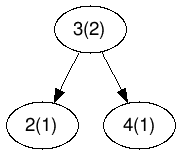
\includegraphics[width=0.3\columnwidth]{fig/bst_duplicate_counter.png}

    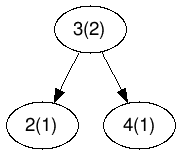
\includegraphics[width=0.3\columnwidth]{fig/bst_duplicate_counter.png}



Python is object-oriented programming language and its underlying implementation is \texttt{C++}, which has a good mapping with the abstract data structures we discussed. Learn how to use Python data type can be learned from the official Python tutorial: \url{https://docs.python.org/3/tutorial/}. However, in order to grasp the efficiency of data structures needs us to examine its C++ source code (\url{https://github.com/python/cpython}) that relates easily to abstract data structures.




\subfile{chapters/chapter_3_iteration_recursion}
\label{chapter_iteration_recursion}



\subfile{chapters/chapter_15_bit-manipulation}
\label{chapter_bit}

\subfile{chapters/chapter_code_data_structure}
\label{chapter_code_data_strucutres}


% \subfile{chapters/chapter_code_graph_and_tree}
% \label{chapter_code_graph_and_tree}


% \subfile{chapters/chapter_searching_strategies}
% \label{chapter_searching_strategies}


%%%%%%%%%%%%%%%%
% Part Two: Principle %
%%%%%%%%%%%%%%%%
\part{Core Principle: Algorithm Design and Analysis}
\label{part_core_principles}
This part embodies the principle of algorithm design and analysis techniques--the central part of this book. 

Before we start, I wanna emphasize that \textbf{tree} and \textbf{graph} data structure, especially tree, is a great visualization tool to assist us with algorithm design and analysis. Tree is a recursive structure, it can almost used to visualize any recursive based algorithm design or even computing the complexity in which case it is specifically called \textit{recursion tree}.  


The next three chapters we introduce the principle of algorithm analysis(chapter~\ref{chapter_algorithm_analysis}) and fundamental algorithm design principle--Divide and conquer(Chapter.~\ref{chapter_divide_conquer}) and Reduce and conquer(Chapter.~\ref{chapter_decrease_and_conquer}). In Algorithm Analysis, we familiarize ourselves with common concepts and techniques to analyze the performance of algorithms -- running time and space complexity. Divide and conquer is a widely used principle in algorithm design, in our book, we dedicate a whole chapter to its sibling design principle --reduce and conquer, which is essentially a superset of optimization design principle--dynamic programming and greedy algorithm--that is further detailed in Chapter.~\ref{chapter_dynamic-programming} and Chapter.~\ref{chapter_greedy}. 



\subfile{chapters/chapter_5_algorithm_analysis}
\label{chapter_complexity_analysis}

\subfile{chapters/chapter_searching_strategies}
\label{chapter_searching_strategies}


\subfile{chapters/chapter_combinatorial_search}
\label{chapter_search_problem_combinatorics}

%chapter 4 divide and conquer
\subfile{chapters/chapter_reduce_and_conquer}
\label{chapter_reduce_and_conquer}

% \subfile{chapter/chapter_searching_strategies}
% \label{chapter_searching_strategies}
\subfile{chapters/chapter_decrease_and_conquer}
\label{chapter_decrease_and_conquer}

\chapter{Sorting and Selection Algorithms}
\label{chapter_sorting}
\subfile{chapters/chapter_14_sorting}



\label{chapter_dynamic-programming}
\subfile{chapters/chapter_12_dynamicprogramming}

% chapter 13
\chapter{Greedy Algorithms}
\subfile{chapters/chapter_13_greedy_algo}
\label{chapter_greedy}

\subfile{chapters/chapter_hands_on_problem_solving}
\label{chapter_hands_on_problem_solving}


%%%%%%%%%%%%%%%%
% Part 4: Advanced Search %
%%%%%%%%%%%%%%%%
\part{Classical Algorithms}
\label{part_classical_algorithms}
In this part, we focus on application through solving a few families of classical real-problems, ranging from advanced search algorithms on linear data structures, advanced graph algorithms, to typical string pattern matching. By studying and analyzing each problem's representative algorithm whereby the fundamental algorithm design and analysis principles are leveraged,  we further enforce our skills to algorithmic problem solving. 
% \label{part_complete_searching}
% \subfile{chapters/part_complete_search_introduction}

\chapter{Advanced Search on Linear Data Structures}
\subfile{chapters/chapter_advanced_linear_search}
\label{chapter_advanced_linear_search}


 \chapter{Advanced Graph Algorithms}
\label{chapter_advanced_searching}
\subfile{chapters/chapter_advanced_graph_algorithm}


\chapter{Advanced Data Structures}
\label{chapter_advanced_data_structures}
\subfile{chapters/chapter_advanced_data_structures}



\chapter{String Pattern Matching Algorithms}
\label{topic_string_processing}
\subfile{chapters/question_2_string_matching}

% \part{Heuristic Search}
% \chapter{Heuristic Search}
% \label{chapter_heuristic_search}
% \subfile{chapters/chapter_heuristic_search}



%%%%%%%%%%%%%%%%
% Part 6: Math abd bit Manipulation %
%%%%%%%%%%%%%%%%
%%%%%%%%%%%%%%%%%%%%%%%%%%%%%%%%%%%%%%%%%%%%%%%%%%%%%%%%%%%%%%%%%%%%%%%%%%%%%%%%%%%%%
%%%%%%%%%%%%% Sorting
% %%%%%%%%%%%%%%%%%%%%%%%%%%%%%%%%%%%%%%%%%%%%%%%%%%%%%%%%%%%%%%%%%%%%%%%%%%%%%%%%%%%%%%%%%
% \part{Combinatorics}
% \label{part_combinatorial_problems}
% % chapter 14




%  \part{Solutions for Exercises}
%  \subfile{chapters/solutions}
%  \label{part_solutions}

% \part{Advanced Algorithms and Data Structures}  
% \label{part_advanced_topics}
% In this part, we would include more detailed topics such as advanced graph algorithms, string process, dynamic programming, backtracking. 
% chapter tree
% \chapter{Advanced Tree Algorithms}
% \label{chapter_advanced_tree_algorithms}
% \subfile{chapters/chapter_12_tree_algorithm}
% chapter 11



% % chapter 15
% \chapter{Bit Manipulation}
% \label{chapter_bit}
% \subfile{chapters/chapter_15_bit-manipulation}
%%%%%%%%%%%%%%%%%%%%%%%%%%%%%%%%%%%%%%%%%%%%%%%%%%%%%%%%%%%%%%%%%%%%%%%%%%%%%%%%%%%%%
%%%%%%%%%%%%% Math and Probability Problems
%%%%%%%%%%%%%%%%%%%%%%%%%%%%%%%%%%%%%%%%%%%%%%%%%%%%%%%%%%%%%%%%%%%%%%%%%%%%%%%%%%%%%%%%%
\part{Math and Geometry}
\label{part_math_bit_manipulation}
% chapter 15

% chapter 16
\chapter{Math and Probability Problems}
\subfile{chapters/chapter_16_math}
\label{chapter_math_probability}

\part{Problem-Patterns}
\label{part_question}

\chapter{Array Questions(15\%)}
\subfile{chapters/question_3_array_question}
\label{array_problem}

\chapter{Linked List, Stack, Queue, and Heap Questions (12\%)} %(44+34+9+31)
\label{other_linear_datastrcutre_problem}
\subfile{chapters/question_4_linked_list_question}


\chapter{String Questions (15\%)}
\label{chapter_string_problem}
\subfile{chapters/question_5_pattern-matching}


\chapter{Tree Questions(10\%)}
\label{chapter_tree_problem}
\subfile{chapters/chapter_13_tree_algorithm}


\chapter{Graph Questions (15\%)}
\label{chapter_graph_problem}
\subfile{chapters/question_7_specific_algorithms_for_graph}

% chapter 1
\chapter{Dynamic Programming Questions (15\%)}
\subfile{chapters/question_1_dynamic_programming}
\label{dp_problem}

 \part{Appendix}
 \chapter{Cool Python Guide}
\subfile{chapters/chapter_introduction_to_python}
\label{appendix_python}

% \suffile{chapters/chapter_introduction_to_python}
% \label{chapter_introduction_to_python}
\nocite{*}
\bibliographystyle{IEEEbib}
{\bibliography{refer}}
\end{document}With $l$ and $r$ to represent the left and right child of node $x$,  there are two other definitions other than the binary search tree definition we just introduced,:  (1)$l.key \leq x.key < r.key$ and (2) $l.key  < x.key \leq r.key$. In these two cases, our resulting BSTs allows us to have duplicates. 

